\documentclass[a4paper, 12pt, oneside]{book}

%\usepackage[utf8x]{inputenc}
\usepackage{times}
\usepackage{verbatim}
\usepackage{color}
\usepackage{url}
\usepackage{graphicx}
\usepackage{array}
\usepackage{mathtools}
\usepackage{algorithm}
\usepackage{algorithmic}
\usepackage{multirow}
\usepackage{tabulary}
\usepackage{subcaption}
\usepackage{lscape}% 將表格橫放
\usepackage{titletoc}% 中文目錄用

% define new columntype from:
% http://tex.stackexchange.com/questions/12703/how-to-create-fixed-width-table-columns-with-text-raggedright-centered-raggedlef
\newcolumntype{C}[1]{>{\centering}m{#1}}

\usepackage{wallpaper}

% uncomment this if you want to indent the first paragraph
%\usepackage{indentfirst}

% uncomment this if you want to make pdf file with hyperlink
% \usepackage[dvipdf,colorlinks=false,unicode]{hyperref}

% uncomment the following and correct them if you want to set
% set the pdf properties
%\hypersetup{
%	pdfauthor={Tz-Huan Huang},
%	pdftitle={A Benchmark for Region-of-Interest Detection in Images},
%	pdfsubject={ddddd}
%}

\usepackage{nccu}
\usepackage{booktabs}
\usepackage{pdfpages}

\setcounter{tocdepth}{2}

\pagestyle{plain}

\usepackage{titlesec}
\titleformat{\chapter}[display]
  {\normalfont\huge\bfseries\centering}{\chaptertitlename\ \thechapter}{20pt}{\Huge}
% 顯示中文章節
\usepackage{CJKnumb}
%\titleformat{\chapter}[display]
%  {\centering\Huge\bfseries}{第\,\CJKnumber{\thechapter}\,章}{1em}{\Huge}

\begin{document}

% cover page
%\CenterWallPaper{}{watermark}
\maketitle
% side page, used for printing on spline.
\makeside

\maketitlep

%\frontmatter

\begin{CJK}{UTF8}{bkai}
\CJKhorz
% 將圖表更改為中文表示
\renewcommand\contentsname{Content}
\renewcommand\listfigurename{Figure Content}
\renewcommand\listtablename{Table Content}
\newcommand{\loflabel}{Figure}
\newcommand{\lotlabel}{Table}
\renewcommand\figurename{Figure}
\renewcommand\tablename{Table}
\renewcommand\bibname{Reference}
%\makecertificationCH
%\makecertificationEN

% comment one of the following unless you are sure you want to
% have both english and chinese acknowledgements in your thesis

%\input{acknowledgementsEN}

%\begin{acknowledgementsCH}

\setlength{\baselineskip}{1.5em}
中文測試
\\
\\
\\
\raggedleft{\textbf{陳XX}}

\raggedright{國立政治大學資訊科學系}

\raggedright{November\ 2016}

\end{acknowledgementsCH}

%\begin{abstractCH}

本篇論文主要在探討如何利用近期所發展之深度學習技術在於中文句子分散式表示法學習。 
近期深度學習受到極大的注目,相關技術也隨之蓬勃發展。然而相關的分散式表示方式,大多以英文為主的其他印歐語系作為主要的衡量對象,也據其特性發展。 
除了印歐語系外,另外漢藏語系及阿爾泰語系等也有眾多使用人口。還有獨立語系的像日語、韓語等語系存在,各自也有其不同的特性。
中文本身屬於漢藏語系,本身具有相當不同的特性,像是孤立語、聲調、量詞等。
近來也有許多論文使用多語系的資料集作為評量標準,但鮮少去討論各語言間表現的差異。\\

本論文利用句子情緒分類之實驗,來比較近期所發展之深度學習之技術與傳統詞向量表示法的差異,也深入探討此些模型對於中文句子情緒分類之表現。

\end{abstractCH}


\begin{abstractEN}

The paper demonstrates how the deep learning methods published in recent years applied in Chinese dataset.

Recently, the deep learning techniques have attracted the great attention. Related areas also grow enormously. 
However, the most techniques use Indo-European languages mainly as evaluation objective, and developed corresponding to their properties.  
Besides Indo-European languages, there are Sino-Tibetan language and Altaic language, which also spoken widely. 
There are only some independant languages like Japanese or Korean, which have their own properties.
Chinese itself is belonged to Sino-Tibetan language family, and has some character like isolating language, tone, count word...etc.
Recently, many publications also use the multilingual dataset to evaluate their performance, but few of them discuss the differences among different languages. 

This study demonstrates the difference from traditional techniques with the preproccess like segmentation, and dive into the models for Chinese. 

\end{abstractEN}


\tableofcontents
% 目錄顯示中文章節
\titlecontents{chapter}[0em]
{}{\makebox[4.1em][l]
{{\thecontentslabel}}}{}
{\titlerule*[0.7pc]{.}\contentspage}
%\end{CJK}
% 將圖表目錄改為圖1.1 表1.1 (Latex預設不會顯示)
\renewcommand{\numberline}[1]{\loflabel~#1\hspace*{1em}}
\listoffigures
\renewcommand{\numberline}[1]{\lotlabel~#1\hspace*{1em}}
\listoftables

\mainmatter

% input your thesis here
\chapter{緒論}
\setlength{\baselineskip}{1.5em}
\setlength{\parindent}{2em}
\setlength{\parskip}{1em}

\section{前言}

How to make the computer can operate the sentence with its own semantics more precisely is study of interest. Since the internet text volume grows so enormously and rapidly, how to make the information can be extracted more efficiently and precisely become more critical for many application. Chinese forums, blogs or microblog grow especially rapidly.    

Recently word2vec is considered to work for evaluated word semantics.  Additionally, the character is invariant to the language. Nevertheless, the problems in sentence level is more complicated, it's related to the sentence structure,  intention or context. There is several methods raised in recent years, like Siamese-CBOW, FastText ...etc. Most of them is able to train batch of text and construct the vectors.

\section{研究目的}

So far, most the studies are conducted in English, we are also interested if the feature also works in Chinese or other languages, and if the algorithm is invariant to the language grammar.
\chapter{Related Work}


\section{Traditional Approach}

\cite{Dashtipour2016} summarized both corpus-base and lexicon-base techniques purposed recently and listed the languages those techniques aiming at, and there are some innovative mothods combined both approaches. 
The advantage of corpus-base is that it is dictionary-free, but it requires relatively larger corpus to build the model, while lexicon-based approach depends mainly on existing resources to detect the sentiment.
When lexicon-based approach comes to the informal articles contributed by netizens, it may suffer some troubles like misspelling, abbreviation ,words or metaphor...etc, neither can it take the sequence of words into consideration.   

The basic corpus-based approach like TF-IDF is considered to be able to generate relatively good precision.
However, both approaches may utilize some keywords in the sentences rather than sentiment of sentence itself. In real world, we often use negation or irony to present our feeling rather than solely keywords. 
To solve the problems from rapidly-evolved languages, there are both semi-supervised and unsupervised approaches introduced as well. 

\section{Chinese Related Sentiment Analysis}

In recent years, most models are aimed at English or more general way. 

When it comes to multiligual environment, the preprocess approach may differ in languages. The traditional ways to counter the variation of words like stemming or lemmatization are appliable to most Latin languages.
Howerver, in Chinese and Japanese, segmentation may also be invloved. In the example of FastText\cite{joulin2016fasttext}, they also demostrated to convert character into pinyin, which make the subword infomation can be obtained. 

Though most approaches are tested and verified by English dataset, there are some work to test in Chinese dataset as well.

\cite{zhao2012moodlens} performed the basic way to classify the articles from WeiBo with Naive Bayes and smoothing with Laplace smooth.  
In this work, the authors also use emoticon as the ground truth to verify the approach, it also applied some imcrement learning. \\

%There are also some researches about Emoticon in sentiment analysis like 
%\cite{Emojis}, which indicates the high correlation between emoticon and sentiment from the users. 

\section{Advanced Approach}

Besides the tradition approaches, which try to extract the effective features. With deep approach, it may be possible to learn more in  continuous representations
Additionally, sentiment analysis with typical deep learning models are conducted, like CNN 
\cite{kim2014convolutional}, RNN \cite{arevian2007recurrent}, but most of them are applied in English dataset only. 

Recently, word2vec(Mikolov et al. 2013)\cite{word2vec} is considered to perform efficiently to vecctorize the meaning of single words. Therefore, the same concept can be adapted to phrase or sentence level as well.
Mikolov also purpose it with sentence level \cite{PVDB}, and claimed it can applied to both short text and long article. These approaches are unsupervised, but it can be conducted to sentiment analysis with proper transformation. 

To detect the sentiment polarity of short text has attracted the interest of study as well, the most used dataset is informal tweet, which is contributed by the netizens from different background. 
For the task of sentiment classification, an effective feature learning method is to compose the representation of a
sentence (or document) from the representations of the words or phrases it contains (Socher et al., 2013b; Yessenalina and Cardie, 2011).

Pang et al. (2002)\cite{pang2002thumbs} already used bag-of-word representation, and present the word as one-hot vector, and they get the better classification results. However, it's still not enough to represent the complex meaning or linguistic characteristics.
The following works, like \cite{tang2014learning}, the paper purpose to use deep learning to do sentiment analysis directly.

There is also a work\cite{multilingual} to evaluate the multiligual approach and monoligual one. However, it used the Spanish and English as target, both two are belongs 
to Indo-European languages. It also addressed the culture difference, "dragon" mean harmful in English but it's opposite in Chinese. 

\chapter{Methods}

\section{The model introduction}

Here are some models we tested, including TF-IDF, fasttext, PVDM, and siamese-CBOW.

\section{TF-IDF + SVM}

	TF-IDF represent as \enquote{term frequency–inverse document frequency}. The conventional way to evaluate the semantics based on the occurrence of words and term, 
  and it also takes the occurrence of word in global context into consideration, which means the more entry the word present, less meaningful it is.

  It is simple and effective, but it still suffers from some disadvantages like data sparsity and high dimension, which may slow down the classifiers, and inability to model synonym. \\

  The SVM we conducted is LinearSVC in sklearn, which uses linear kernel. It used one-vs-rest strategy to handle the multiclass cases.
  In the other word, it generates fewer models than SVC does.
  We used default parameters. The penalty is l2, and loss function is squared hinge. 

\section{Fasttext}
	
The approach is purposed by \cite{joulin2016fasttext}. 
The structure of fasttext can be considered as extension of word2vec as well, and it uses the hierarchical softmax to compute the probabilities for predefined classes. 
However, the key difference of fasttext from word2vec is that it employed bag of N-grams features. 
For example the word vector “apple” is a sum of the vectors of the N-grams “\textless ap”, “app”, ”appl”, “apple”, “apple\textgreater”, “ppl”, “pple”, “pple\textgreater”, “ple”, “ple\textgreater”, “le\textgreater”.
This approach tries to take the local word order into consideration and evaluate the partial information from spelling. It may also vectorize the rare words better, which have less neighboring words to model.
It also a countermeasure to solve the problem of bag-of-words, that the order of words is not considered. 
For example, the terms \enquote{我見你} (I see you) and \enquote{你見我}(you see me) are contributed to the same results in bag of words model.
However, in the ngrams model, the vector are average from its subset, including \enquote{我見}(I see), \enquote{我} (I)...etc, it makes it possible to distinguish the difference.

While the computation and space complexity increase, it employs the hashing trick like word2vec as well. 
The word representation is looked up through a table and finally averaged into the text representation. 
For the words absent from word embeddings, it uses subword infomation\cite{bojanowski2016enriching} to guess the meaning of the word.
Another trick applied is pruning some of the vocabulary elements. Feature selection among N-gram is very inefficient and complicated.
Here it used online parallelizable greedy approach: To check if the document is covered already, if not, add one with highest norm.

Finally it uses the linear classification to classify the data. The classifier called \enquote{Product quantization} uses some tricks to speed up, which utilizes compressed-domain approximate nearest neighbor search (Jegou et al., 2011) \cite{jegou2011searching}.
The compression technique approximates a real-valued vector by finding the closest vector in a pre-defined structured set of centroids like Figure \ref{fig:pq}.
The original PQ has been concurrently improved by Ge et al. \cite{ge2013optimized} and Norouzi \& Fleet , who learn an orthogonal transform minimizing the overall quantization loss.
The technique may scrifice some accuracy to gain much more performance and efficiency of memory. It is proved by their experiment that with normalization, both PQ and OPQ are almost lossless with 4 subquantizers. 

We used the released version from Facebook github.

\begin{figure}[h]
    \centering
	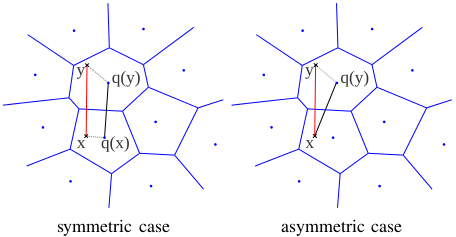
\includegraphics[width=.8\linewidth]{pq}
    \caption{Production quantization: It use predefined centroids to proximate the distance of 2 points. There are two type of PQ, symmetric and asymmetric. }
    \label{fig:pq}
\end{figure}

\begin{figure}[h]
    \centering
	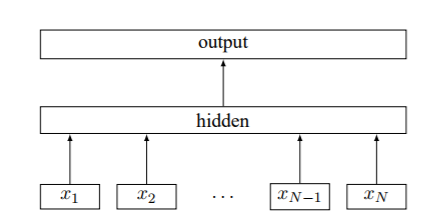
\includegraphics[width=.8\linewidth]{fasttext}
    \caption{The architecture of fasttext: the image is cited from \cite{joulin2016fasttext}.}
    \label{fig:fasttext}
\end{figure}


\section{Paragraph Vector}
	
The method is purposed in \cite{PVDM}. The idea is to obtain the summary of paragraphs, sentences or documents. 
There are 2 different algorithms they purposed, which are distributed memory(DM) and distributed bag of words(DBOW). 
The DM model in figure \ref{fig:dm} is quite similar with word2vec. The difference between PVDM and word2vec is that the former contains paragraph matrix.
Every paragraph is mapped to unique vector. Figure \ref{fig:dbow} show the model architecture. Compared with DM model, DBOW is conceptually simple, this model store less data. 

The paragraph vectors are asked to contribute to the prediction task of the next word given many contexts sampled from the paragraph.
The contexts are fixed-length and sampled from a sliding window over the paragraph. Therefore, DM take the sequence into consideration.

However, in DBOW model, it ignores context words from input and forces the model to predict words randomly sampled from the paragraph in the output.
It is quite similar to Skip-gram in word2vec.

The author suggested that DM is consistently better in general cases, while DBOW take fewer resources. 
Two models also can be concatenated, which means combine both models together. 
The author claimed it is applicable to both short sentence and long paragraph.\\

We use the implementation of Gensim and use SVM with linear kernel to classify.

\begin{figure}
\centering
\begin{subfigure}{.5\textwidth}
  \centering
  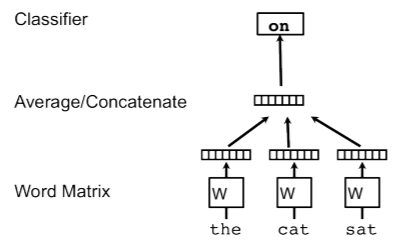
\includegraphics[width=.9\linewidth]{dm}
  \caption{distributed memory}
  \label{fig:dm}
\end{subfigure}~
\begin{subfigure}{.5\textwidth}
  \centering
  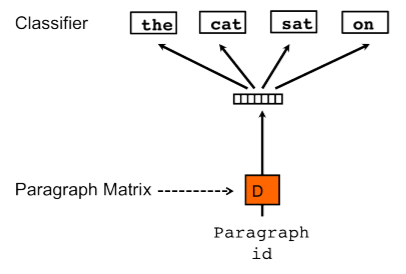
\includegraphics[width=.9\linewidth]{DBOW}
  \caption{distributed bag of words}
  \label{fig:dbow}
\end{subfigure}
\caption{Paragraph vector: the images show the difference of two models, and the images are from \cite{PVDM}.}
\label{fig:PVDM}
\end{figure}

\section{Siamese-CBOW}

	The Simese-CBOW\cite{kenter2016siamesecbow} computes sentence embeddings is to average the embeddings of its
constituent words, instead of using pre-trained word embedding. 

It applied the concept of bag of word from word2vec. It used the average from the words composing the sentence and use it to evaluate the possibility to predict the sentence around. 
The architecture shows as Figure \ref{fig:siamese}. As it indicated, the word embeddings are optimized directly for averaging.
A supervised training criterion by predicting sentences occurring next to each other in the training data.
Cosine similarities are used to compute the proximity of sentences.
Softmax is applied in the last layer to produce the final probability distribution.

The author also evaluated the effect of the hyperparameters. The number of negative sampling yield limited loss, and the higher dimension is preferred to generate better result.

We used the implementation (https://bitbucket.org/TomKenter/siamese-cbow/overview) from the author, and made it compatible with python3 for better compatibility with unicode.

\begin{figure}[h]
    \centering
	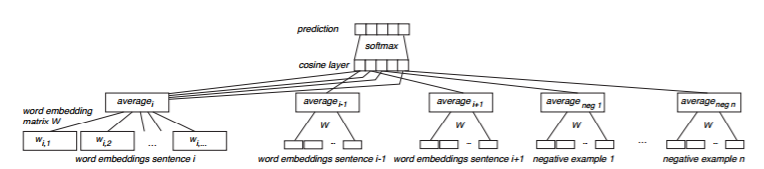
\includegraphics[width=.9\linewidth]{siamesecbow}
    \caption{The architecture of Siamese-CBOW, the image is from original paper\cite{kenter2016siamesecbow}.}
    \label{fig:siamese}
\end{figure}

\chapter{Experiment}

\section{Set Up}

\begin{table}[]
\centering
\caption{Tag Category}
\label{CategoryTable}
\begin{tabular}{|c|c|}
\hline
JOY  & 呵呵 酷 \begin{CJK}{UTF8}{gbsn}赞 乐乐\end{CJK} 贊 鼓掌 耶 \\
DISGUST & \begin{CJK}{UTF8}{gbsn}黑线 汗 晕\end{CJK} \\
SAD &   可憐 淚 衰 失望 \begin{CJK}{UTF8}{gbsn}伤心 泪\end{CJK} 生病 囧 \begin{CJK}{UTF8}{gbsn}鄙视\end{CJK}  \\
FEAR &  委屈  可憐 \\
SURPRISE &  吃驚  \begin{CJK}{UTF8}{gbsn}吃惊\end{CJK} \\
ANGER & 怒 抓狂 \\
\hline
\end{tabular}
\end{table}

\begin{figure}[h]
    \centering
	
\includegraphics[width=1\linewidth]{weibo}
    \caption{The emoticons in WeiBo}
    \label{fig:weibo}
\end{figure}

The dataset we chose is Open WeiboScope\cite{fu2013reality}, which is collected WeiBo randomly with API by researchers at the Journalism and Media Center of the University of Hong Kong in 2012. 
It contains 226 millions posts distributing evenly over the year.  
The most weibo users come from the different province of China. There are also some users from Hong Kong or oversea. 
The content of weibo contains both simplified Chinese and traditional Chinese. Some province dialect also can be seen in the dataset.

It's a Weibo feature to allow the user to use emoticon, 
and the emoticon in raw data expressed as [笑](smile),[淚](tear). It displays as images like the Figure \ref{fig:weibo}. 
We used the tags in posts as the indicators of sentiment, and removed some duplicated posts or some posts without any tags, or too many tags. 
We evaluated the accuracy of the classification for different algorithms. We used the TF-IDF and SVM (Joachims, 1998). as baseline.

\section{Preprocess}

For the data preprocessing and cleansing, most posts contains more than 1 tag. To avoid ambiguity, we only preserve those with single tag.
we removed the posts containing too many tags, or without any tag. We also removed the duplicated posts by their post id roughly because it is a property of Chinese microblog \cite{fu2013reality} for Chinese netizens to post repeatedly. 
Besides, we only chose the posts over certain length (over 10 characters). Finally, we used jieba and dictionary to segment to post. \\

We used most-used 6 emotion which most social network support: JOY, SAD, ANGER, FEAR, SURPRICE, DISGUST.
We classify these tags into these classes manually. 
Like \cite{zhao2012moodlens}, we also suffered the problem that the numbers of emoticon classes skewed. The numbers of JOY and SAD are more than 50\% of posts. 
We only selected some specific tags from JOY and SAD to make the whole dataset more balance.   
The mapping table shows in Table \ref{CategoryTable}. The JOY contains the tags like 呵呵(haha), 贊(excellent)...etc. 
The SAD contains the tags like 失望(disppointed), 淚(tear).


We removed the tags from the original post, and there are so many tags. 
The posts left for 6 categories display in Table \ref{cat_num}. The majority classes are still JOY and SAD. 

After initial round, we found some special string or tokens like username or url may affect the result. 
Therefore, we also removed those special tokens from the posts as well.

\begin{table}[]
\centering
\caption{Number for categories}
\label{cat_num}
\begin{tabular}{|c|c|}
\hline
ANGER      &331,091 \\                                                           
DISGUST    &261,955 \\                                                         
FEAR       &151,564 \\                                                         
JOY        &717,059 \\                                                           
SAD        &788,492 \\                                                           
SURPRICE   &191,974 \\
\hline
\end{tabular}
\end{table}


\section{PVDM}

In the Paragraph vector experiment, we tested both DM and DBOW. Additionally, there are 2 different DM supported by gensim to use average or concatenation.
We use DM/C and DM/M to represent concatenation and average separately, and used the parameters suggested for 3 models. 

The dimension is 100, and negative-sampling is 5 for both DM and DBOW models, and window size are 5, 10 for concatenation, average separately. 

\section{FastText}

In the FastText experiment, we tried 3 formats, including non-segmented dataset, segmented dataset and the dataset with pinyin.
We tested the non-segmented dataset, since some training data in demostration is Japanese without segmentation. We wonder if the segmentation matters.
Additionally, we also want to test if the subword information work for Chinese. So we convert the dataset to pinyin as well. We can see the differences from the table\ref{ftdataset}.

For converting to pinyin, we use jieba + pinyin (https://www.npmjs.com/package/pinyin) npm package to convert the  charaters to pinyin, which also includes the tone.
We used built-in classifier to classify the test set.

\begin{table}[]
\centering
\caption{FastText Dataset}
\label{ftdataset}
\begin{tabular}{|c|c|}
\hline
   & \\
\hline
no segmentation  & 弊喇,好似有少少喉嚨痛添! \\
segmentation  & 弊 喇 , 好似 有 少 少 喉嚨痛 添 ! \\
segmentation + pinyin  & bì lǎ , hǎosì yǒu shǎo shǎo hóulóngtòng tiān ! \\
\hline
\end{tabular}
\end{table}

We also tested the both dimesion size from 8-300, and loss function including hs (Hierarchical Softmax), ns (negative sampling), softmax.


\section{Siamese-CBOW}

In the siamese-cbow, we use siames-cbow with the default parameters that the author suggested. 
The dimension is 100, and update algorithm is ada delta. 
We ran it with epoch 5, 10 separately without any pre-trained word embedding, so it generates the word embedding from scratch.
Due to low performance of the trial without pre-trained word embedding, we also tried to use gensim to generate the pre-train word embedding from our dataset.
With pre-trained word embedding, we tried epoch 10 to run.

After the vectors are generated, we use both multinomial Naive-Bayes and Linear SVC to classify the results.
\chapter{Conclusion}

\begin{table}[]
\centering
\caption{Results}
\label{resultAll}
\begin{tabular}{|c|c|}
\hline
Tf-IDF   & 0.44 (± 0.04) \\
PVDM(dbow) & 0.40    \\
FastText &  ~0.51   \\
FastText(Pinyin) &  ~0.51  \\
Siamese-CBOW(5) & 0.41 (± 0.04) \\
Siamese-CBOW(10) & 0.39 (± 0.03) \\
Siamese-CBOW(10) with pre-train & 0.45 (± 0.02) \\

\hline
\end{tabular}
\end{table}

\begin{table}[]
\centering
\caption{FastText}
\label{fasttext}
\begin{tabular}{|c|c|c|c|c|c|}
\hline
   & 8 & 12 & 16 & 32 & 64 \\
\hline
no segmentation  & 0.369 & 0.375 & 0.389 & 0.372 & 0.368 \\
segmentation  & 0.515 & 0.515 & 0.514 & 0.516 & 0.513 \\
segmentation + pinyin  & 0.513 & 0.518 & 0.516 & 0.517 & 0.51 \\
\hline
\end{tabular}
\end{table}

\begin{table}[]
\centering
\caption{Result of PVDB}
\label{resultAll}
\begin{tabular}{|c|c|c|c|}
\hline
      & Test set & Training Set \\
\hline
dm/c  & 0.384 &  0.384 \\
dbow &  0.404  & 0.457 \\
dm/m &  0.38  & 0.436 \\
\hline
\end{tabular}
\end{table}


\section{Experiment Settings}


We used baseline TD-IDF plus SVM with linear kernel as baseline. 
Since the original distribution for classes is a little skewed, most the test sample is classified into 2 major classes.
We compared it with other models with different settings. \\

For PVDB, we use 3 different models dm/c and dm/m and dbow. All of them, we choose most commonly-used parameters,dm : dimension:100, window size:10, negative:5, hs:0 and we tested both dm with concatenation of context vectors (dm/c) and average of context vectors(dm/m). 
The other model dbow, we chose the same parameters.

In FastText experiment, we iterated through the parameters like window size from 8 to 100, 
loss function ns,hs,softmax.  Since the result did't indicate significant difference between these parameters, 
we only display 1 of them as reference.

Additionally, we also tried to convert data set to pinyin to evaluate 
if the pinyin improve the sematic recognition for FastText, 
which support vocabulary expansion with subword information \cite{bojanowski2016enriching}. 

\section{Result}

It took around 2 days with GPU NVIDIA TITAN X (PASCAL) to finish Siamese-CBOW word-embedding training. With both 5,10 epoch the perforamance are below the baseline. 
We would discuss in the Discussion. The other models can be complete with CPU within hours.

We also look into the classification result with confusion matrix in Figure \ref{confusion1} and Figure \ref{confusion2}.

That we can see that the 2 major classes get best accuracy while the test results skewed into these 2 major classes as well.  
The ANGER, DISGUST, and FEAR are more likely to be classified as SAD. It is reasonable that those posts contain more negative feeling.
The tendancy in the Siamese-CBOW result is more obvious. And it classify no entry into some rarely-used classes.

\begin{figure}[h]
    \centering
	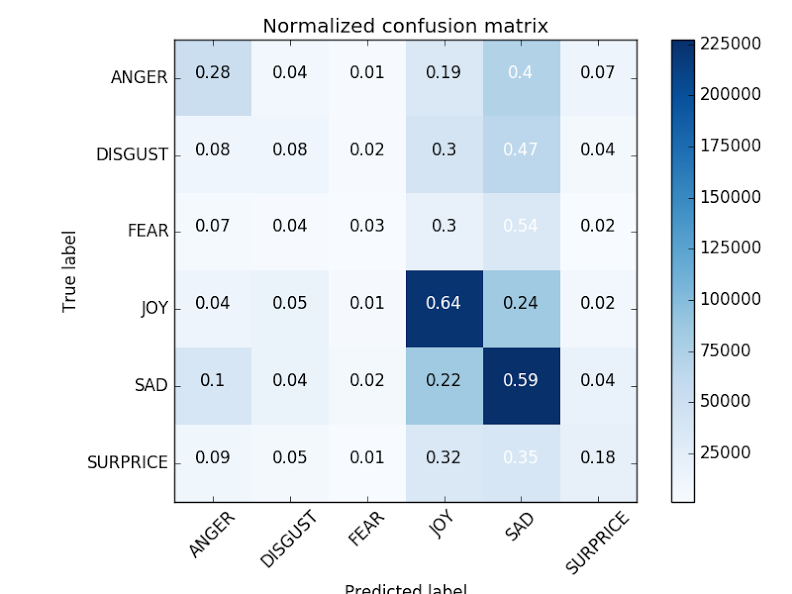
\includegraphics[width=1\linewidth]{tf-idf}
    \caption{The confusion matrix for TF-IDF+ SVM}
    \label{confusion1}
\end{figure}

\begin{figure}
\centering
\begin{subfigure}[b]{1\textwidth}
   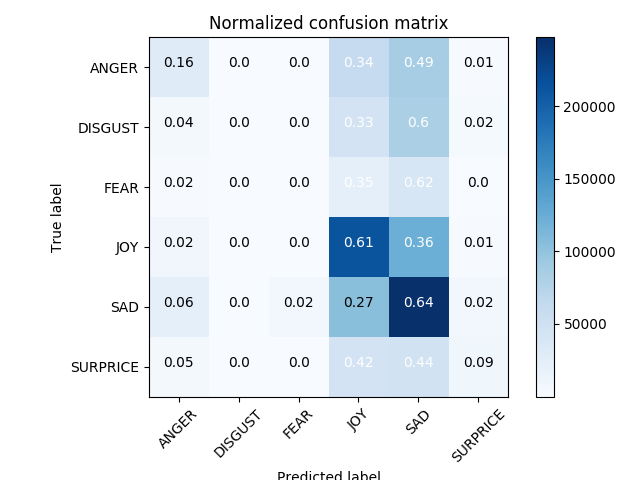
\includegraphics[width=.9\linewidth]{sc-ratio}
   \caption{}
   \label{confusion2} 
\end{subfigure}

\begin{subfigure}[b]{1\textwidth}
   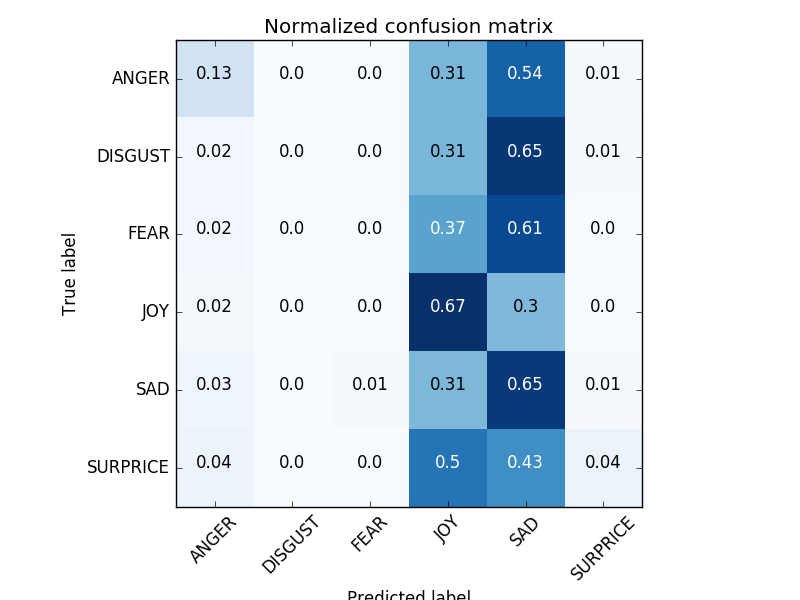
\includegraphics[width=.9\linewidth]{siamese-cbow-pretrained}
   \caption{}
   \label{confusion5}
\end{subfigure}
\caption[Confusion Matrix of Siamese-CBOW]{(a) The training set without pre-trained embedding,
(b) The training set with pre-trained embedding
}
\end{figure}


In the confusion matrix for fasttext in Figure \ref{confusion4}, it shows different tendancy for Pinyin dataset classification. 
The accuracy for SURPRICE is higher than SAD. It indicates that the SURPRICE may be modeled better than SAD, which contains more sample.

Figure \ref{confusion4} is quite similar with other confusion matrix, where most test data are classified as JOY and SAD.

\begin{figure}
\centering
\begin{subfigure}[b]{1\textwidth}
   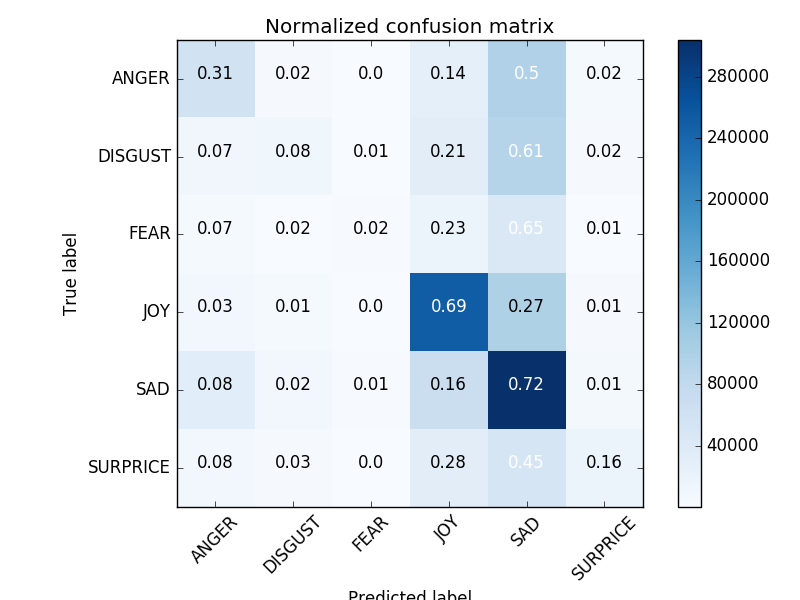
\includegraphics[width=.9\linewidth]{fasttext-All_seg_d300_w20_hs}
   \caption{}
   \label{confusion3} 
\end{subfigure}

\begin{subfigure}[b]{1\textwidth}
   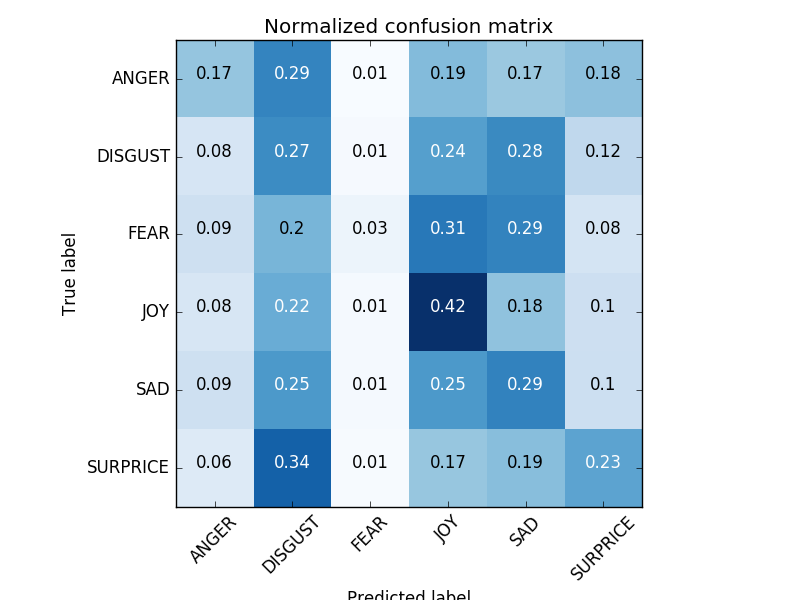
\includegraphics[width=.9\linewidth]{All_seg_d200_w15_softmax_pinyin}
   \caption{}
   \label{confusion4}
\end{subfigure}
\caption[Confusion Matrix of FastText]{(a) segmented dataset trained with dimension=300, window size=20, loss function hierarchical softmax,
(b) pinyin dataset with dimension=200, window size=15, and loss function = softmax
}
\end{figure}

\chapter{Discussion}

The result shows that FastText can archive better accuracy in general way. We also compare the result between different models.

\section{Discussion}


For the baseline, though TF-IDF it can archive the accuracy about 0.44(±0.04). 
The most distinguishable features they use are some rarely used terminology. 
Since we only removed the duplicated post roughly, it may still suffer from the duplicated post from different sources with certain rarely-used words. 
In general, the model is not general enough, it may not be applicable when the data set changed. 

Additionally, compared to other methods, those approaches convert the sentence to vectors with lower dimensions.
Theoretically, it may benefit the classifier with more dense presentation. Sparse matrix cause much more time and space to train.
With such high dimension vectors, it is unlikely to apply the non-linear classifier.

Generally, FastText can retrieve the better accuracy with segmentation inclusion, and is able to train the large-scale dataset more efficiently with its own classifer.
With conversion to Pinyin, it also achieves the similar accuracy. Though, we tried the different settings for FastText,
the accuracy is not different significantly despite of the various settings of loss function, window size and dimensions. 
In the comparison set, segmented dataset outperforms the one without segmentation. 
It suggested that the term itself may be more meaningful than a single character. And it also took much less time than that of other implementatons.
Although we did not perform it with linear classifier like that in other experiments, we can consider that the accuracy is not lossless.

\section{Baseline}

\begin{CJK}{UTF8}{gbsn}
We used TF-IDF as baseline, the result is 0.44(±0.04), which is statistically greater than the random result in 6 classes problem, 
even we consider the skewed classes.  We tried to evaluate the feature that TF-IDF use to classify as Table \ref{table:featureoftfidf}. 
Though some term here seemed related like, 2nd place in ANGER is \begin{CJK}{UTF8}{bkai}造謠\end{CJK} (create humor),3rd one is 恶浪(violent billow). 
The 2nd place in FEAR is 谋财害命(commit murder for money). The most term is not so related intuitively. 
\end{CJK}

Most of words in each classes actually are not used so commonly. It is contributed by the problem of IDF, which may overweight some rarely-used words.
The other problem is that we observed the netizen keep posting something quite similar like advertisement, joke or news..., 
Though their content are not the same exactly, the words or terminology they used may be quite common. 
Besides TF-IDF, most algorithms assume that the articles themselves are distinct from others. In real world, it is not a common case except some well-organized website articles.
We may require some extra preprocess procedure to handle to prevent intentionally repeated posts.

Some publications\cite{Chen2013TUP25129382512940} shows that the posters may use some morphs to avoid censorship, which we can't evaluate how these words contributes to the sentiment analysis. 
However, the similarity of morphs is quite easy to identified by Word2vec with proper context. 
It is relatively difficult to identify in TF-IDF model. 
\begin{CJK}{UTF8}{gbsn}
\begin{table}[]
\centering
\caption{The feature extracted from TF-IDF}
\label{table:featureoftfidf}
\begin{tabular}{|c|c|c|c|c|c|}
ANGER	& DISGUST	& FEAR	& JOY	& SAD	& SURPRICE \\
\hline
想瘦	&抬杠	&含铅	&余则	&grunewald	&印钞机 \\
\begin{CJK}{UTF8}{bkai}造謠\end{CJK}	&赃款	&谋财害命	&符离	&节省时间	&绝密\\
恶浪	&由此看来	&表同情	&驻守	&张春桥	&54:03.7\\
顶缸	&淫妇	&经济体	&神明	&前导	&清福\\
银行利息	&\begin{CJK}{UTF8}{bkai}觀天象\end{CJK}	&\begin{CJK}{UTF8}{bkai}可憐見\end{CJK}	&asce	&\begin{CJK}{UTF8}{bkai}已閱\end{CJK}	&任免\\
卫冕冠军	&解除	&突如其来	&三元里	&q1050505041	&karei\\
落水狗	&上刑	&万念俱灰	&何苦来哉	&杀伐	&一桩\\
剖腹自杀	&矢泽爱	&供应站	&太妙了	&离世	&sikucd\\
剥下	&超现实主义	&\begin{CJK}{UTF8}{bkai}勞資\end{CJK}	&两面三刀	&\begin{CJK}{UTF8}{bkai}噴火龍\end{CJK}	&touchsmart610\\
多吉	&\begin{CJK}{UTF8}{bkai}美國使館\end{CJK}	&深红	&slient	&\begin{CJK}{UTF8}{bkai}查無此人\end{CJK}	&翻筋斗
\end{tabular}
\end{table}
\end{CJK}

\section{Siamese-CBOW}

\begin{CJK}{UTF8}{gbsn}
The Siamese-CBOW, the performance is below the baseline. We tried evaluate the model it trained, it seemed it is not converged enough. 
The word embedding is not converted correctly. For example, we use \enquote{我} (I) to query in the word-embedding generated by Siamese-CBOW 5 epoch. 
The related words it show are 扙(hurt, rarely-used word),第四节 (the fourth quarter) and 贾宝玉(the name in the novel). With 10 epoch word embedding, the  
related words are 几家 (Some homes), 峯(peek), and 速成班 (rapid-archieve class). It seemed there is no sign of converge.
\end{CJK}

In the confusion matrix, we found the most tested result fall into two major classes.
It is quite similar as other models due to data imbalance.

We tried to use pre-trained word-embeddings with 10 epoch to improve it, and the result is improved to the level of baseline.
However, when we assessed the embeddings it generated, the embeddings are still far from converging. 
According to original paper, the proper embedding can be trained properly. 
We are not sure if the property is not available in Chinese dataset.

In the original paper, the dataset they conduected is Toronto Books, which contains novels,
 therefore the sematics of the sentences may be more highly coherent with previous sentence and next one. 
The property of the dataset should not affect the word embedding it trains. 
However, it may affect how it determines the relationship between sentences in our cases.

Using some pre-trained embeddings may help to improve the performance. 
Another drawback is that Siamese-CBOW does not support the feature like subword information.
It means if the words is absent from its training dataset, it would be consider non-existent at all. Conducting the vocabulary expansion like that in Skip-Thoughts may assist the problem.


\section{PVDM}

In paragraph vector experiment, the result shows that DBOW produced best accuracy among 3 models. In the original paper, the author suggested that the DM is consistently better than DBOW
, and that the sum version of DM is often better than concatenation. 
So far, it is not clear under what condition that DBOW outperform the DM model. We tried leverge the model it built. 
We fetched most similar word of I (我) as Table \ref{table:doc2vec}. Surprisingly, the similar words of DBOW are all not related words. 
Both DM/C and DM/M generated better results, which top 10 related words are synonyms of I.
It seemed predictable that DBOW stored less data to train. DM/C and DM/M actually model the word in more proper way though the accuracy their accuracy is not good.
Though the result is better for DBOW, it may not be robust result. We need more different datasets to evaluate further.
\begin{CJK}{UTF8}{gbsn}
\begin{table}[]
\centering
\caption{The most similar 5 words of I (我) in 2 models of PVDM}
\label{table:doc2vec}
\begin{tabular}{|c|c|c|c|}
\hline
      & DM/C & DBOW & DM/M \\
\hline
1 & 俺 &  三条  & 偶\\
2 & 偶  & 田徑運動 & 他\\
3 & 老子  & 温暖人间 & 俺\\
4 & 哀家  & youtudou & 我们\\
5 & 皮下  & 化妝水 & 她 \\
\hline
\end{tabular}
\end{table}
\end{CJK}

\begin{table}[]
\centering
\caption{Similar words with \enquote{nǐ}(you) in Pinyin dataset}
\label{table:py_similar}
\begin{tabular}{|c|c|}
\hline
 word related  & Chinese  \\
\hline
wǒ         &   我(I)  \\
nǐzìjǐ     &   你自己(yourself) \\   
nǐmén      &   你們(you)   \\
,"nǐ       &   ,"你(,"you)  \\ 
shuí       &   誰(who)   \\
shuítāmā   &   誰他媽(who in the hell)\\   
wǒhuì      &   我會(I can)   \\
,"shuí     &   ,"誰(who)   \\
,"shuítāmā &   ,"誰他媽(who in the hell)\\   
biérén"    &   別人(others)\\
\hline
\end{tabular}
\end{table}


\section{FastText}

In fasttext, we tried to evaluate the 3 different datasets, segmented, non-segmented and pinyin. 
Although pinyin dataset archieve the same overall accuracy similar to segmented one, the confusion matrix show different tendancy.
Despite of the various settings of loss function, window size, both segmented dataset and non-segmented one classified most entries into 2 major classes.
While with some specific parameters, the classifier on pinyin dataset can classify the minor class as well. 

We tried to validate the property of vectors generated by pinyin dataset with FastText cbow and skip-gram as Table \ref{table:py_similar}. 
It approves that both cbow and skip-gram can generate the pinyin word-embedding efficiently. 
However, for the non-segmented dataset, the word-embeddings consists vectors of single characters, they are not able use subword information neither.

The other finding about word vector it generated. Some segmented dataset contains some poorly segmented term like \enquote{坑爹}(cheating me),\enquote{有木有}(if or not)... 
, which are new internet language so can not be handled properly by dictionary file, are segmented as separate characters.  
While the word2vec can merge those characters together due to the high occurance of these characters. 
Somehow, fasttext treat them as separate term but they may be related highly.

We tried to use T-SNE to visualize the vector space in Figure \ref{tsne}. As we can see, the vector space with some ambiguous boundary.


\begin{CJK}{UTF8}{gbsn}
\begin{table}[]
\centering
\caption{words with low norm in 3 dataset in fasttext}
\label{table:lownorm}
\begin{tabular}{|c|c|}
\hline
 dataset  & words  \\
\hline
segmented  & \begin{CJK}{UTF8}{bkai} 旳\end{CJK}, 颂, 硬伤, \begin{CJK}{UTF8}{bkai}財\end{CJK}, 索取, 图像, 巾 \\
non-segmented  & 喝水还那么麻烦, 给我试试好么@亚瑟小狼狗....etc   \\
pinyin     &         
\includegraphics[width=0.5\linewidth]{pinyin} \\   
\hline
\end{tabular}
\end{table}
\end{CJK}

\begin{figure*}[t!]
    \centering
     
    \begin{subfigure}[t]{0.5\textwidth}
        \centering
        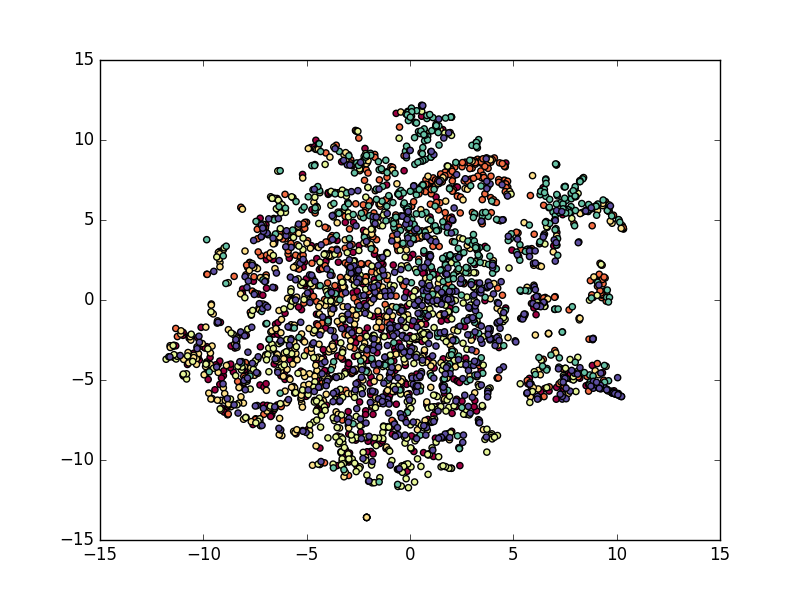
\includegraphics[width=1\linewidth]{ft-All_seg_d200_w15_hs}
        \caption{segmented dataset, dimesion=200 , window size=15, loss function=  hierarchical softmax}
    \end{subfigure}%
    ~
    \begin{subfigure}[t]{0.5\textwidth}
        \centering
        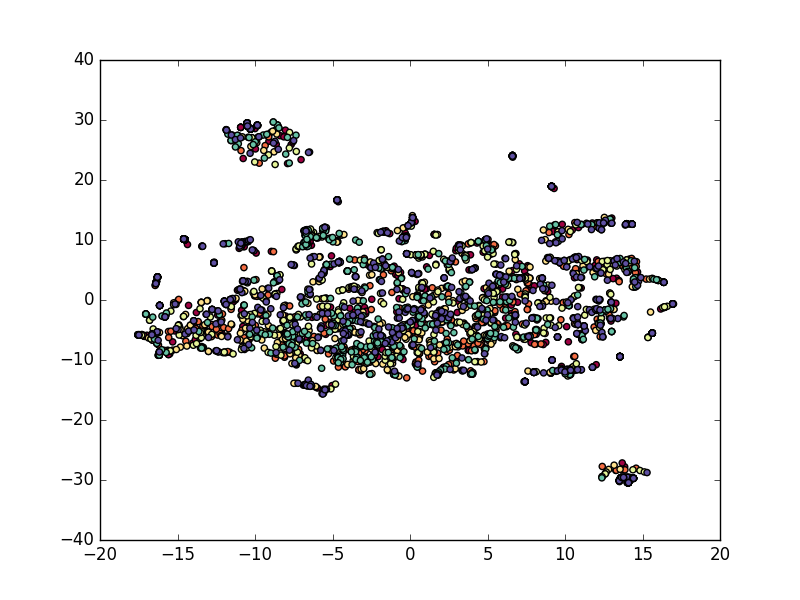
\includegraphics[width=1\linewidth]{fasttext-py-All_seg_d200_w15_softmax_pinyin}
        \caption{pinyin dataset,  dimesion=200 , window size=15, loss function= softmax}
    \end{subfigure}
    \caption{Visualization of vector space for 2 dataset}
    \label{tsne}
\end{figure*}


We tried to analyze the vectors it generate. The number of vectors generated with 3 dataset with 100,000 posts are 25,743, 3,137 and 22,233 for segmented, non-segmented and pinyin dataset separately. 
We listed the vectors with lowest norm in Table \ref{table:lownorm}. As the paper indicated that the vector with lower norm, it contains less infomation. 
Therefore, most of them are stop words. Surprisingly, the non-segmented dataset contains much less words than other 2. 
Additionally, the most words it contains are like the sentences rather than the terms. It implied that the fasttext itself can not handle segmentation properly, and explains why it performs poorly. 
For the segmented dataset, the vectors with lowest norm are some rare used words, which can not be modeled properly with low occurance and few neighboring words around.
For the pinyin dataset, the vectors with lowest norm are those special abbreviation and icons. Compared with segmented dataset, those rare used word may have the the same pronunciation with other words or can be inferred from subword information.

%The other property of fasttext is that it is insensitive to sequence of word order in the sentence.

\subsection{N-grams Evaluation}

We evaluated the vectors from ngram level. We found that the term like \enquote{我們}(our) generated by 4 vector: \enquote{我們}, \enquote{\textless 我們}, \enquote{我們\textgreater}, \enquote{\textless 我們\textgreater} in the segmented dataset,
while the counterpart in the pinyin dataset consist 15 vectors, including \enquote{wǒmén}, \enquote{\textless wǒ}, \enquote{\textless wǒm}, \enquote{\textless wǒmé}, \enquote{\textless wǒmén}...etc. 
The segmented n-grams vectors do not contain single character like \enquote{我}, \enquote{們}, becasuse the setting for prefix or subfix for english consist more than 2 or 3 letters above.

We tried to evaluate the word \enquote{我們的}(ours) in both segmented vectors and pinyin vectors in Table \ref{table:ngrams-seg} and Table \ref{table:ngrams-pinyin}. 
We can see the pinyin contain much more conbinations, and the term \enquote{wǒmén-de} which segmented properly indicated high promixity to the complete term. 
In the segmented set, we can see the same tendancy. \enquote{們的}, the term segmented poorly, generate negative similarity. 

The length of ngrams is limited in 3-5 in this experiment. It may be better to model single character in Chinese by shortening the ngram minimum length.
Additionally, the some pinyin may be consituted by only 2 letters.  Lowering the minimum length may model them better as well, but it may also contribute the extra computation effort.
The length of prefix and suffix may vary depending on the languages, so it may be the parameter we can optimize fasttext depends on the language.

\begin{table}[]
\centering
\caption{ngrams constitution of \enquote{我們的}(ours)}
\label{table:ngrams-seg}
\begin{tabular}{|c|c|}
\hline
 key  &  similarity \\
\hline
\textless我們的\textgreater     &  0.02 \\
\textless我們的     &  0.09 \\
我們的\textgreater     &  0.07 \\
們的\textgreater     &  -0.07 \\
我們的     & 0.19   \\
\textless我們     &  *0.99   \\   
\hline
\end{tabular}
\end{table}

\begin{table}[]
\centering
\caption{ngrams constitution of \enquote{wǒménde} (ours) in pinyin}
\label{table:ngrams-pinyin}
\begin{tabular}{|c|c|}
\hline
 key  &  similarity \\
\hline
\textless wǒ -  ménde\textgreater      &  0.73 - 0.14 \\
\textless wǒm -  énde\textgreater      &  0.70 - 0.19 \\
\textless wǒmé - nde\textgreater     &  0.70 - 0.26 \\
\textless wǒmén - de\textgreater      &  0.70 - 0.62\\
wǒmén      &  0.70 \\
  ménde     & 0.16   \\
mén     &  0.35   \\   
\hline
\end{tabular}
\end{table}

\subsection{Subword Information}

According to the paper, the feature of subword information can compensate the insufficience of word embeddings. 
We tried to evaluate if the features work in pinyin as well, which means sentimatics can be inferred from the pronunciation. 
Although we converted the dataset to pinyin, the accuracy is not significantly different from the original accuracy. 
Intuitively, pinyin is less readible to native speaker and not reversible to the characters, since the multiple characters own the same pronunciation. 
Chinese contains less syllables and more homonyms than English do. In the original paper\cite{bojanowski2016enriching}, they evaluate the effectiveness in various languages like Arabic, Czech, German, English...etc.
All of them belong to phonography, and most languages belong to phonography. While Chinese belongs to logogram specially. 

We tried some examples in segmented and pinyin dataset in Table \ref{table:related-words}
The term acquired shared some similarity in consitute characters, so their meaning are similar by some degree. 
It can not prove the model can assess the sematic of a new term precisely by its consitute character.
For \enquote{\begin{CJK}{UTF8}{gbsn}给力\end{CJK}} (it works or supports), "ok" may be close in some degree, but others are not.
In the example of pinyin seemed only return the terms with morphological similarity.
So far, we are still hard to quantize the effectiveness conducted in Chinese.

In the \cite{MikolovLS13}, it also provides similar function to compensate the words absent from training set. 
It employs similarity of pre-trained word-embedding by mapping the pre-trained space to pre-trained one to expand its vocabulary. 
There are also some differnet approaches like morphologically annotated data, whcih were introduced by Cotterell and Schütze (2015).
It is a good topic to evaluate the difference of these approaches. 

\begin{CJK}{UTF8}{gbsn}
\begin{table}[]
\centering
\caption{Query the word non-existing in dataset}
\label{table:related-words}
\begin{tabular}{|c|c|c|}
\hline
 吃不起 & 给力 & gōngxǐfācái(恭喜發財)  \\
\hline
吃不饱  & ok & gōngxǐ (恭喜)\\
买不起  & 得意 & gōngqíjùn (宫崎骏)\\
吃不完     &  [ & gōngpū(公布)\\   
上不起     &   lt & gōngrè(公认) \\   
经不起     &   想念 & gōngpó(公婆)\\
\hline
\end{tabular}
\end{table}
\end{CJK}

\section{Conclusion}

We demonstrated the various modern methods on the Chinese corpus, and it indicated that PVDM and FastText are invariant to language property. 
In general, most models improve the sematic analysis compared with tranditional TF-IDF, and it is more efficient to extract the information with more dense vectors.
Different models can be used in different context.

Most methods are developed based on English or Latin languages property, so segmentation or other peroprocess work play crucial roles to make other language genaralized.
But the segmentation may also contribute something wrong. Though some of them also can be conducted with non-segmented sentences, it performed worse due to improper segmentation.

We can see FastText demostrate excellent property in both performance including training and testing time and memory utilization. 
Besides the accuracy of the sematic conversion, both the performance and the efficiency of memory also become the interest of study.



\backmatter

%\addcontentsline{toc}{chapter}{\bibname}
\bibliographystyle{abbrv}

% input your reference here
\bibliography{thesis}
\end{CJK}

\appendix

\end{document}
